\section{Accounts and Enrollments}

\subsection{Login and Sign Up}
\textbf{Design}

The login and sign up pages are the first pages the user will see when interacting with the Meta Learning Management System. As such, it needs to be easy to understand while also highly functional. To achieve this, a style that resembles what has become the standard login and sign up procedure across the entire web has been used. On the login screen, a user is prompted for their email address and password, and have a sign in button to submit these credentials for verification. As for the sign up page, the form is similar in format, except with more fields to take in the required information to create a new user account. In addition to requiring a user to enter their email and password, the sign up for also asks for a full name, their student ID, and a password confirmation to ensure that the password they are entering is correct.

\begin{figure}[h!]
    \centering
    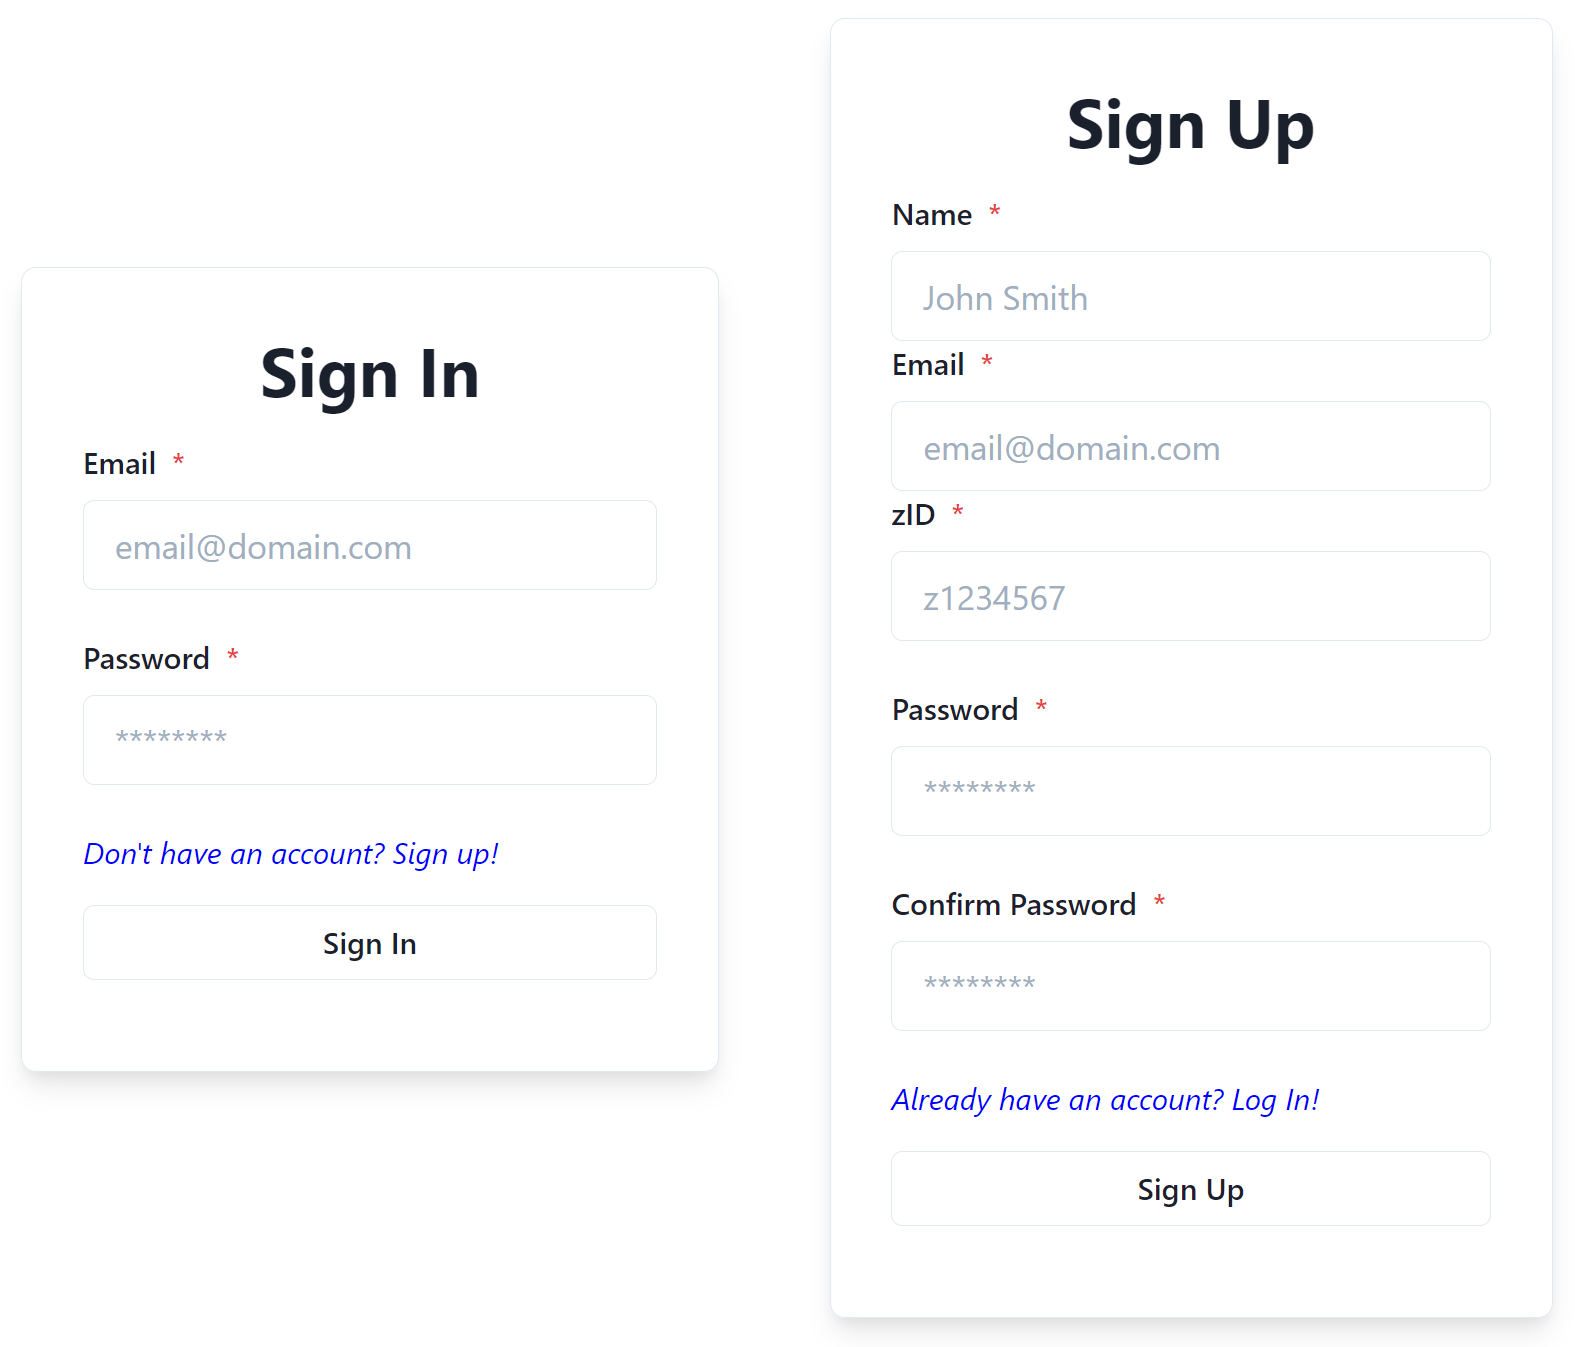
\includegraphics[scale=0.25]{images/accounts-login.png}
    \caption{Login and Sign Up Forms}
\end{figure}

\textbf{Purpose}

By allowing users to create personal accounts within the LMS, it allows all of the other functionality of the LMS to be tailored specifically to that user. The accounts feature is what ties all of a user's progression within their courses to that users, and without it the rest of the LMS would not function.

\textbf{What Was Implemented}

Two forms have been created, a log in form that asks for the users email and password, and a sign up form that asks for a name, email, student ID, password and password confirmation. The inputs on these two forms are text fields that automatically sanitise inputs to ensure they meet the correct formatting, and there is a submission button at the bottom of the form. There is also a hyperlink that allows the user to switch between the sign up and log in context.

\textbf{How It Was Implemented}

The log in for and sign up forms both contain a number of text fields for user input. For log in, the user fills in their log in credentials, their email and password, and submits them. The site then passes this data to the backend, which first searches for that email to confirm it exists within the database, then compares the submitted password to that users password to see if they got the correct credentials. In the case of a failure, it will return an error to the front-end, however on a successful login, it returns a token to the front-end which must then be used with all future requests to the backend to authorise said requests. This token is stored in the browsers storage alongside the users ID, which is also necessary for many of the requests.

The sign up form operates very similarly, except instead of confirming the email already exists in the database, it instead confirms that the submitted email and student ID do not currently exists in the database, then confirms that both the password and confirm password fields both contain the same data. If all of these checks pass, the data is entered into the database, and an authorisation token and user ID are returned to the front-end, the same as the log in form. 

\textbf{Considerations}

A lot of detail was also put into creating intuitive error messages on the login form that are informative to the user, without compromising the security of the Meta LMS. For example, an error message will tell you when a field is missing/has been left blank, but if either the email or password is typed incorrectly, it will simply state ``Incorrect email or password" so as to not reveal to a potential bad actor whether an email address they have entered is in our database or not.

\begin{figure}[h!]
    \centering
    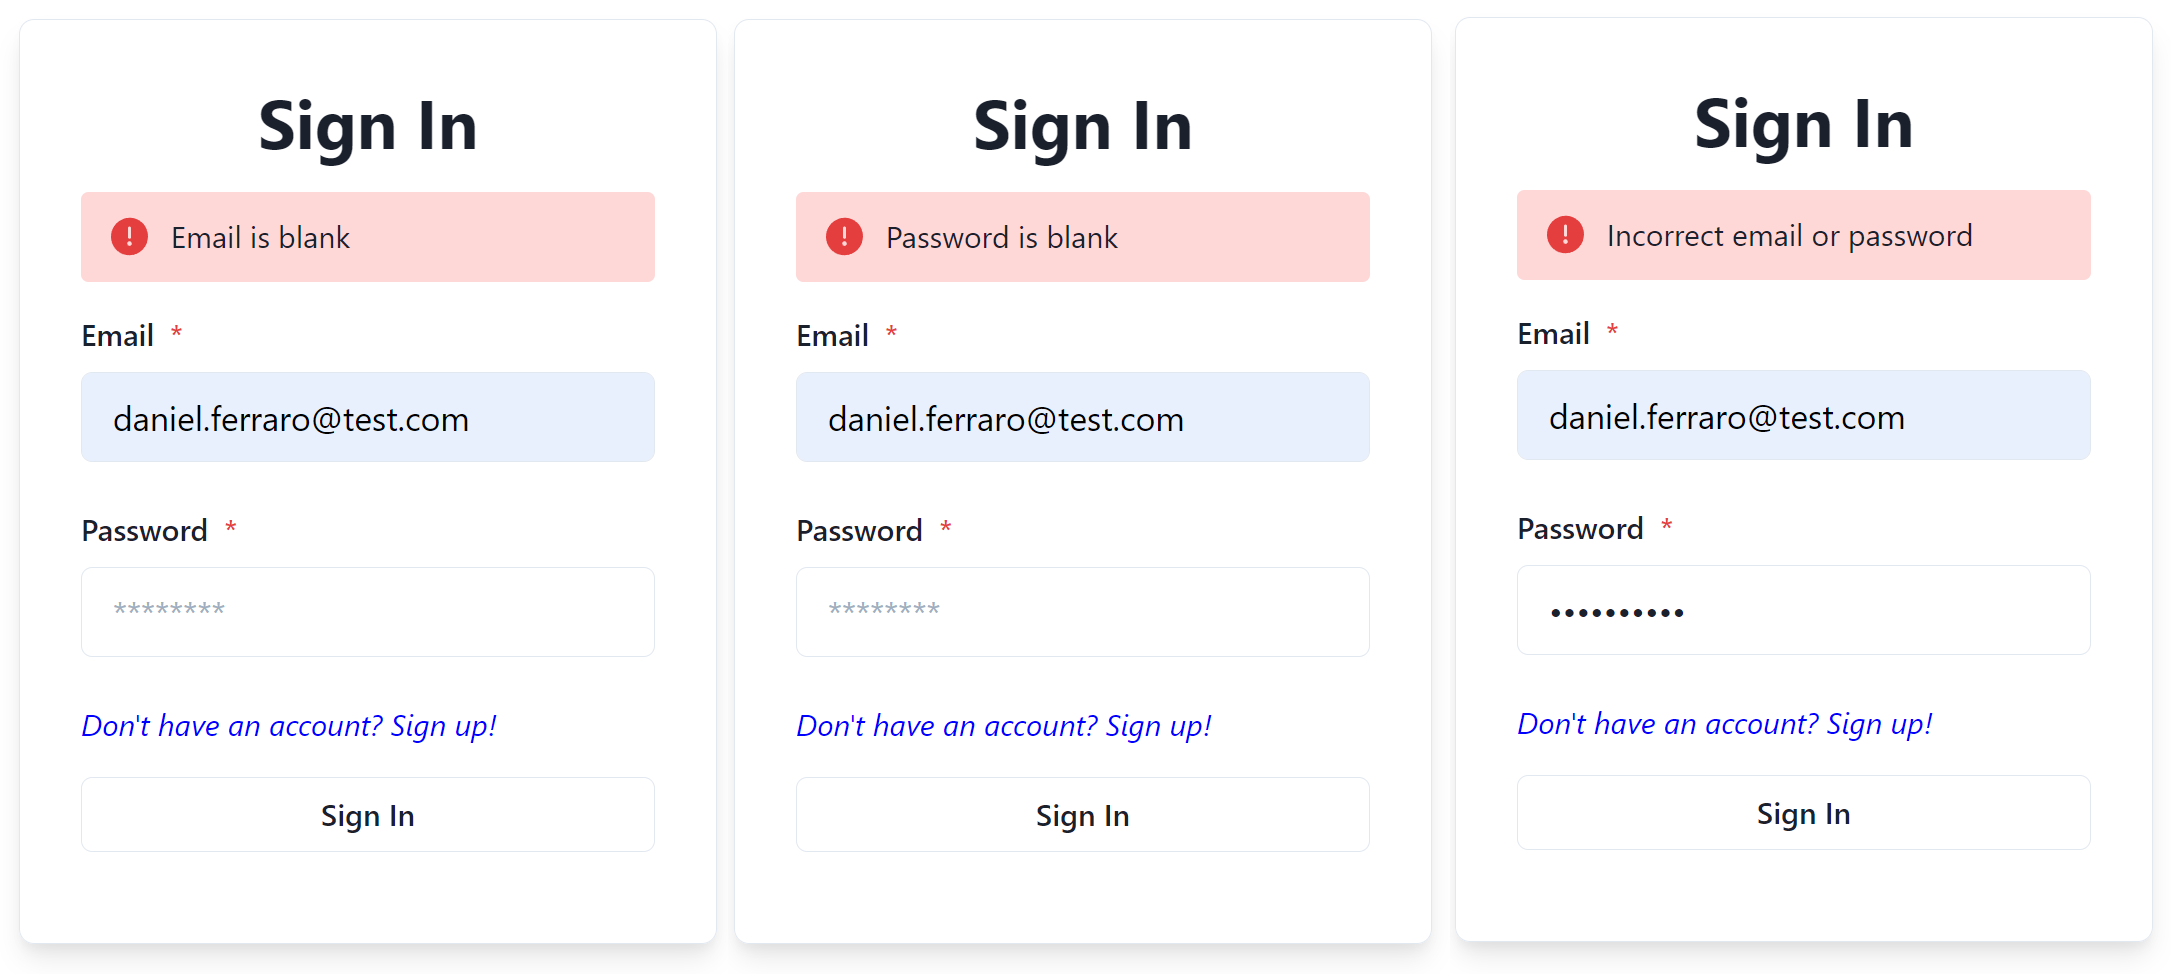
\includegraphics[scale=0.15]{images/accounts-login-errors.png}
    \caption{Login Form Errors}
\end{figure}

\subsection{Account Management}
\textbf{Design}

The account management screen allows users to view and edit their account information easily within the Meta LMS. This page is accessed from the drop-down menu attached to the profile indicator in the top right of the home page. This drop-down also houses the log out button, which when pressed logs out a user and returns them to the log in screen.

\begin{figure}[h!]
    \centering
    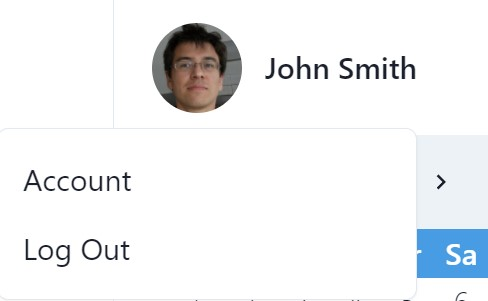
\includegraphics[scale=0.4]{images/accounts-account-dropdown.jpg}
    \caption{Profile Drop-down}
\end{figure}

On the account management screen, a user is shown their full name, student ID and account type, either staff or student, in the page header. They are then show a list of fields that contain their other account information, such as email and profile image URL. Under these fields, is a table showing the courses they are currently enrolled in, in the form of a table showing the course code, course name and course outline. There is also an edit button attached to the account information fields that allows a user to edit their profile.

\begin{figure}[h!]
    \centering
    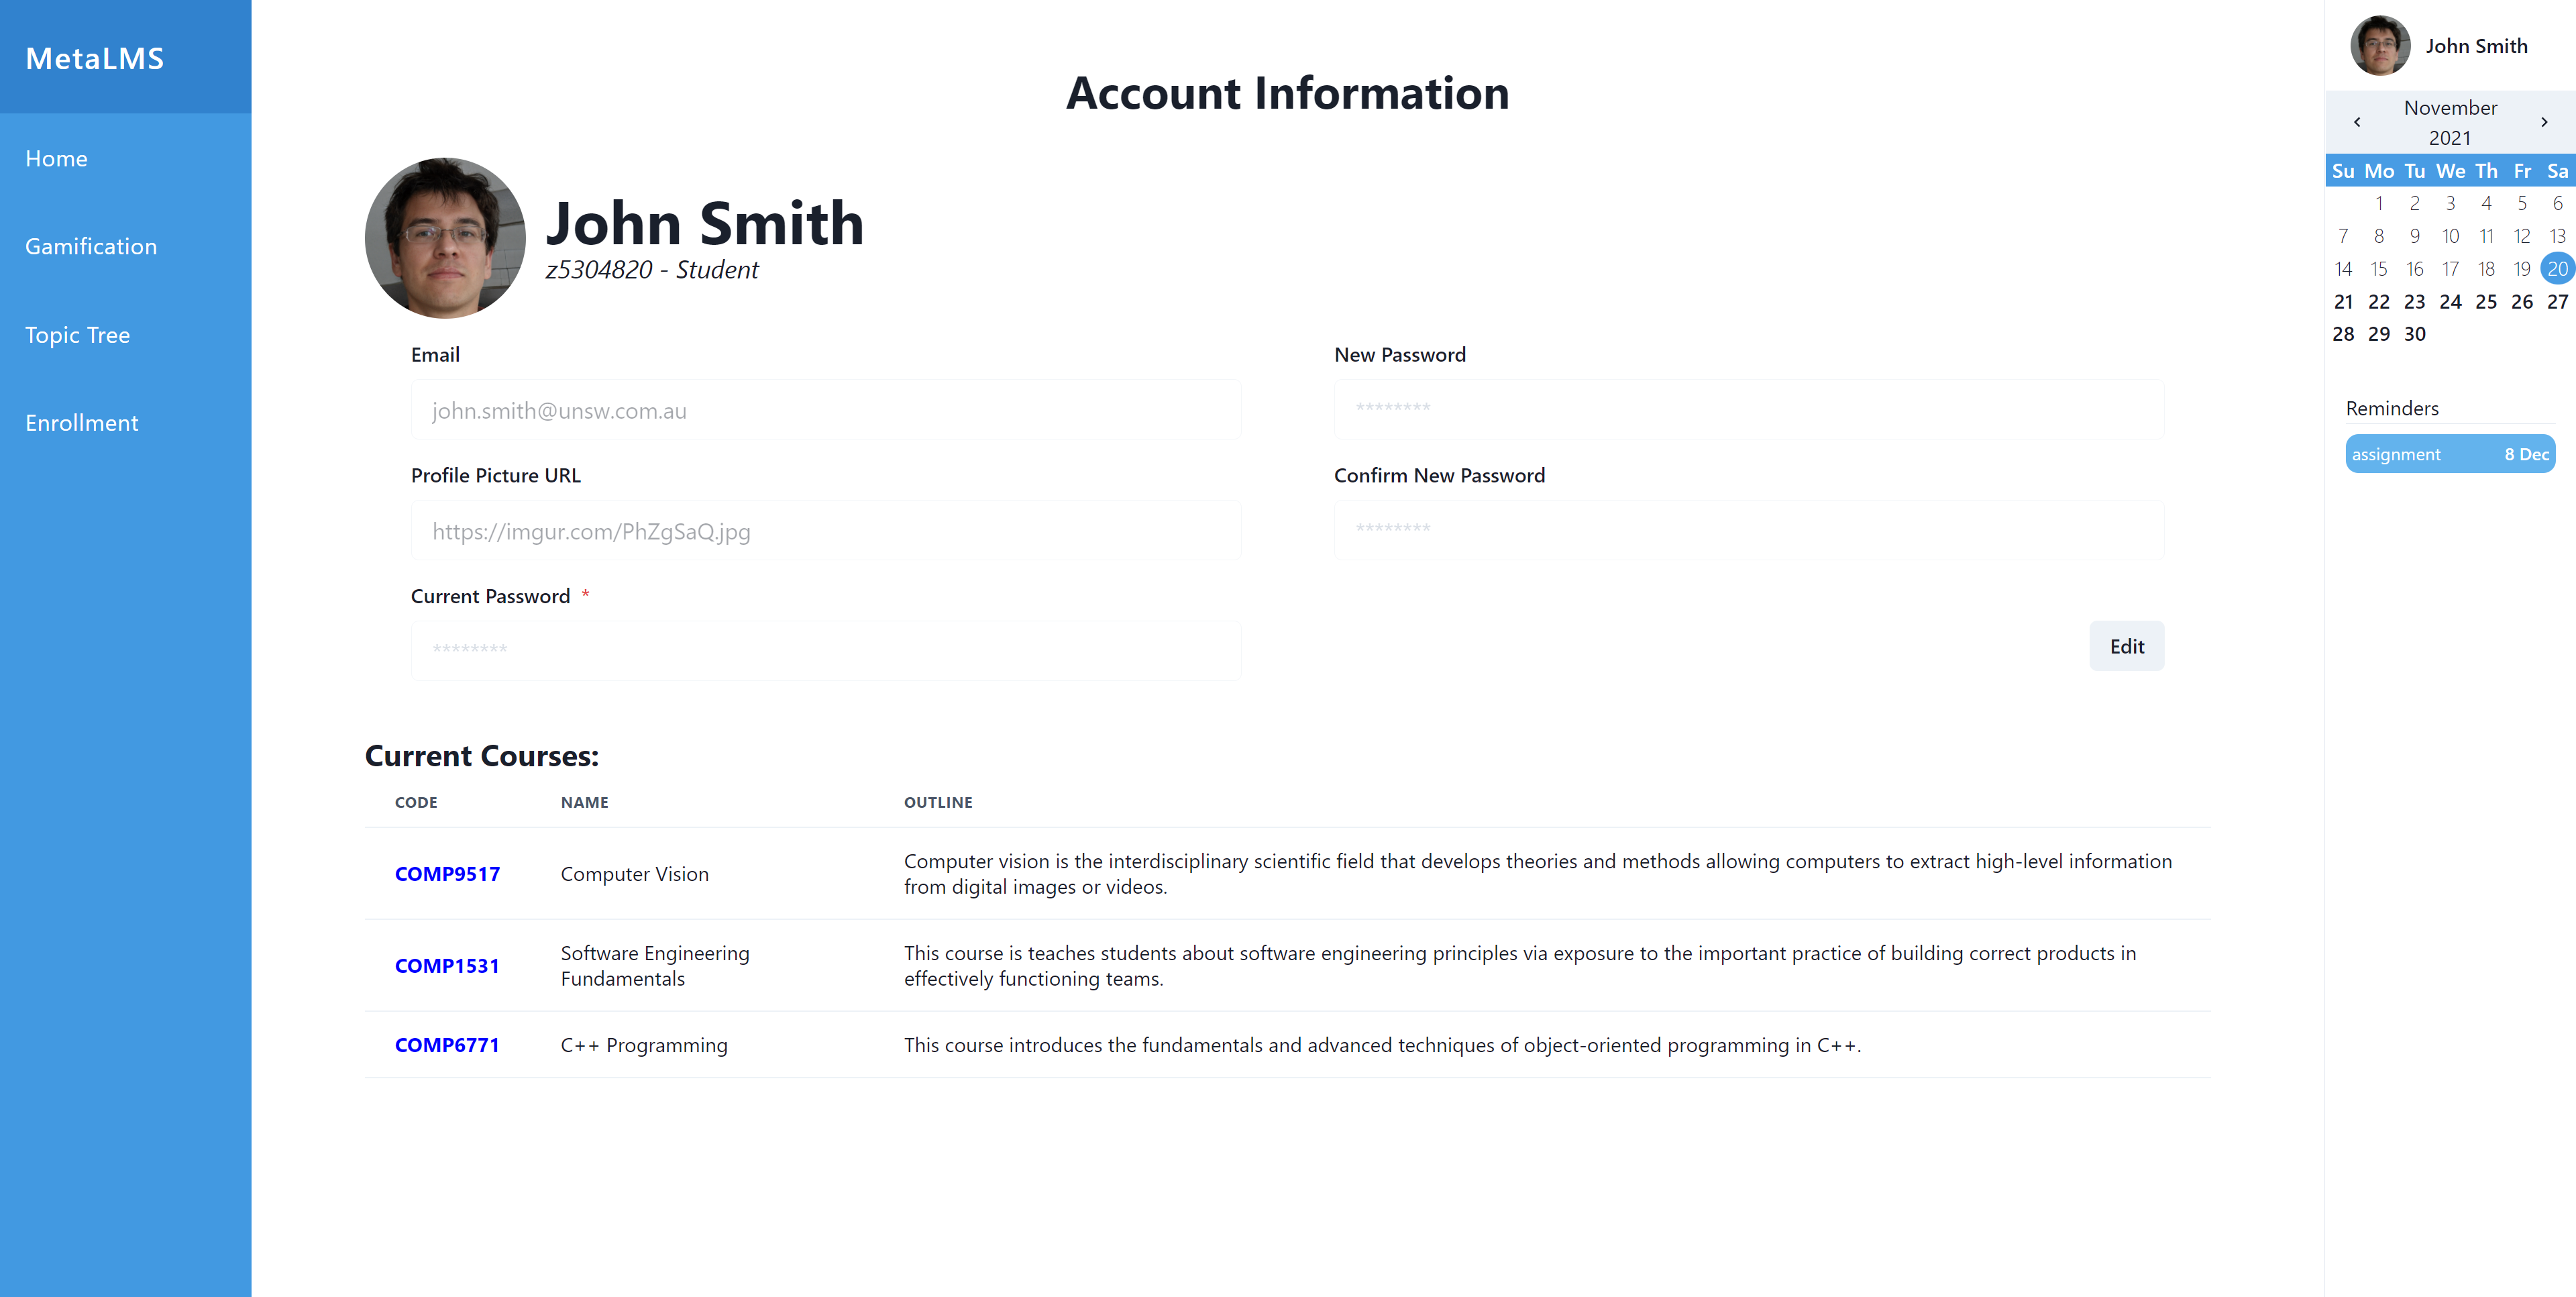
\includegraphics[scale=0.1]{images/accounts-account-management.png}
    \caption{Account Management}
\end{figure}

\textbf{Purpose}

The intention of the account management screen is to have a place within the LMS where the user can view all of the information associated with their account, as well as edit and update this information. By the inclusion of this feature, users have a quick and easy way to ensure all of their personal information is correct and up to date, increasing the user satisfaction as this allows the Meta LMS to remain personalised to the user. It is also a useful tool for quickly viewing all current courses a user is enrolled in or is managing.

\textbf{What Was Implemented}

The accounts screen not only displays all of a users information, there is also an edit button attached to these fields. When clicked, it changes these fields to mutable text boxes, and the edit button changes to a save and cancel button. To edit their account information, a user must mutate the field they wish to change, and also enter their current password to pass the security check required to make the changes. If a user wishes to change their password, they must enter their current password, their new password, then re-enter their new password to confirm it. To change their email, they must simply enter a correctly formatted email, and to change their profile image, they must enter a URL for an image. When these changes are saved, all of the information is quickly updated on the page to reflect these changes. 

\begin{figure}[h!]
    \centering
    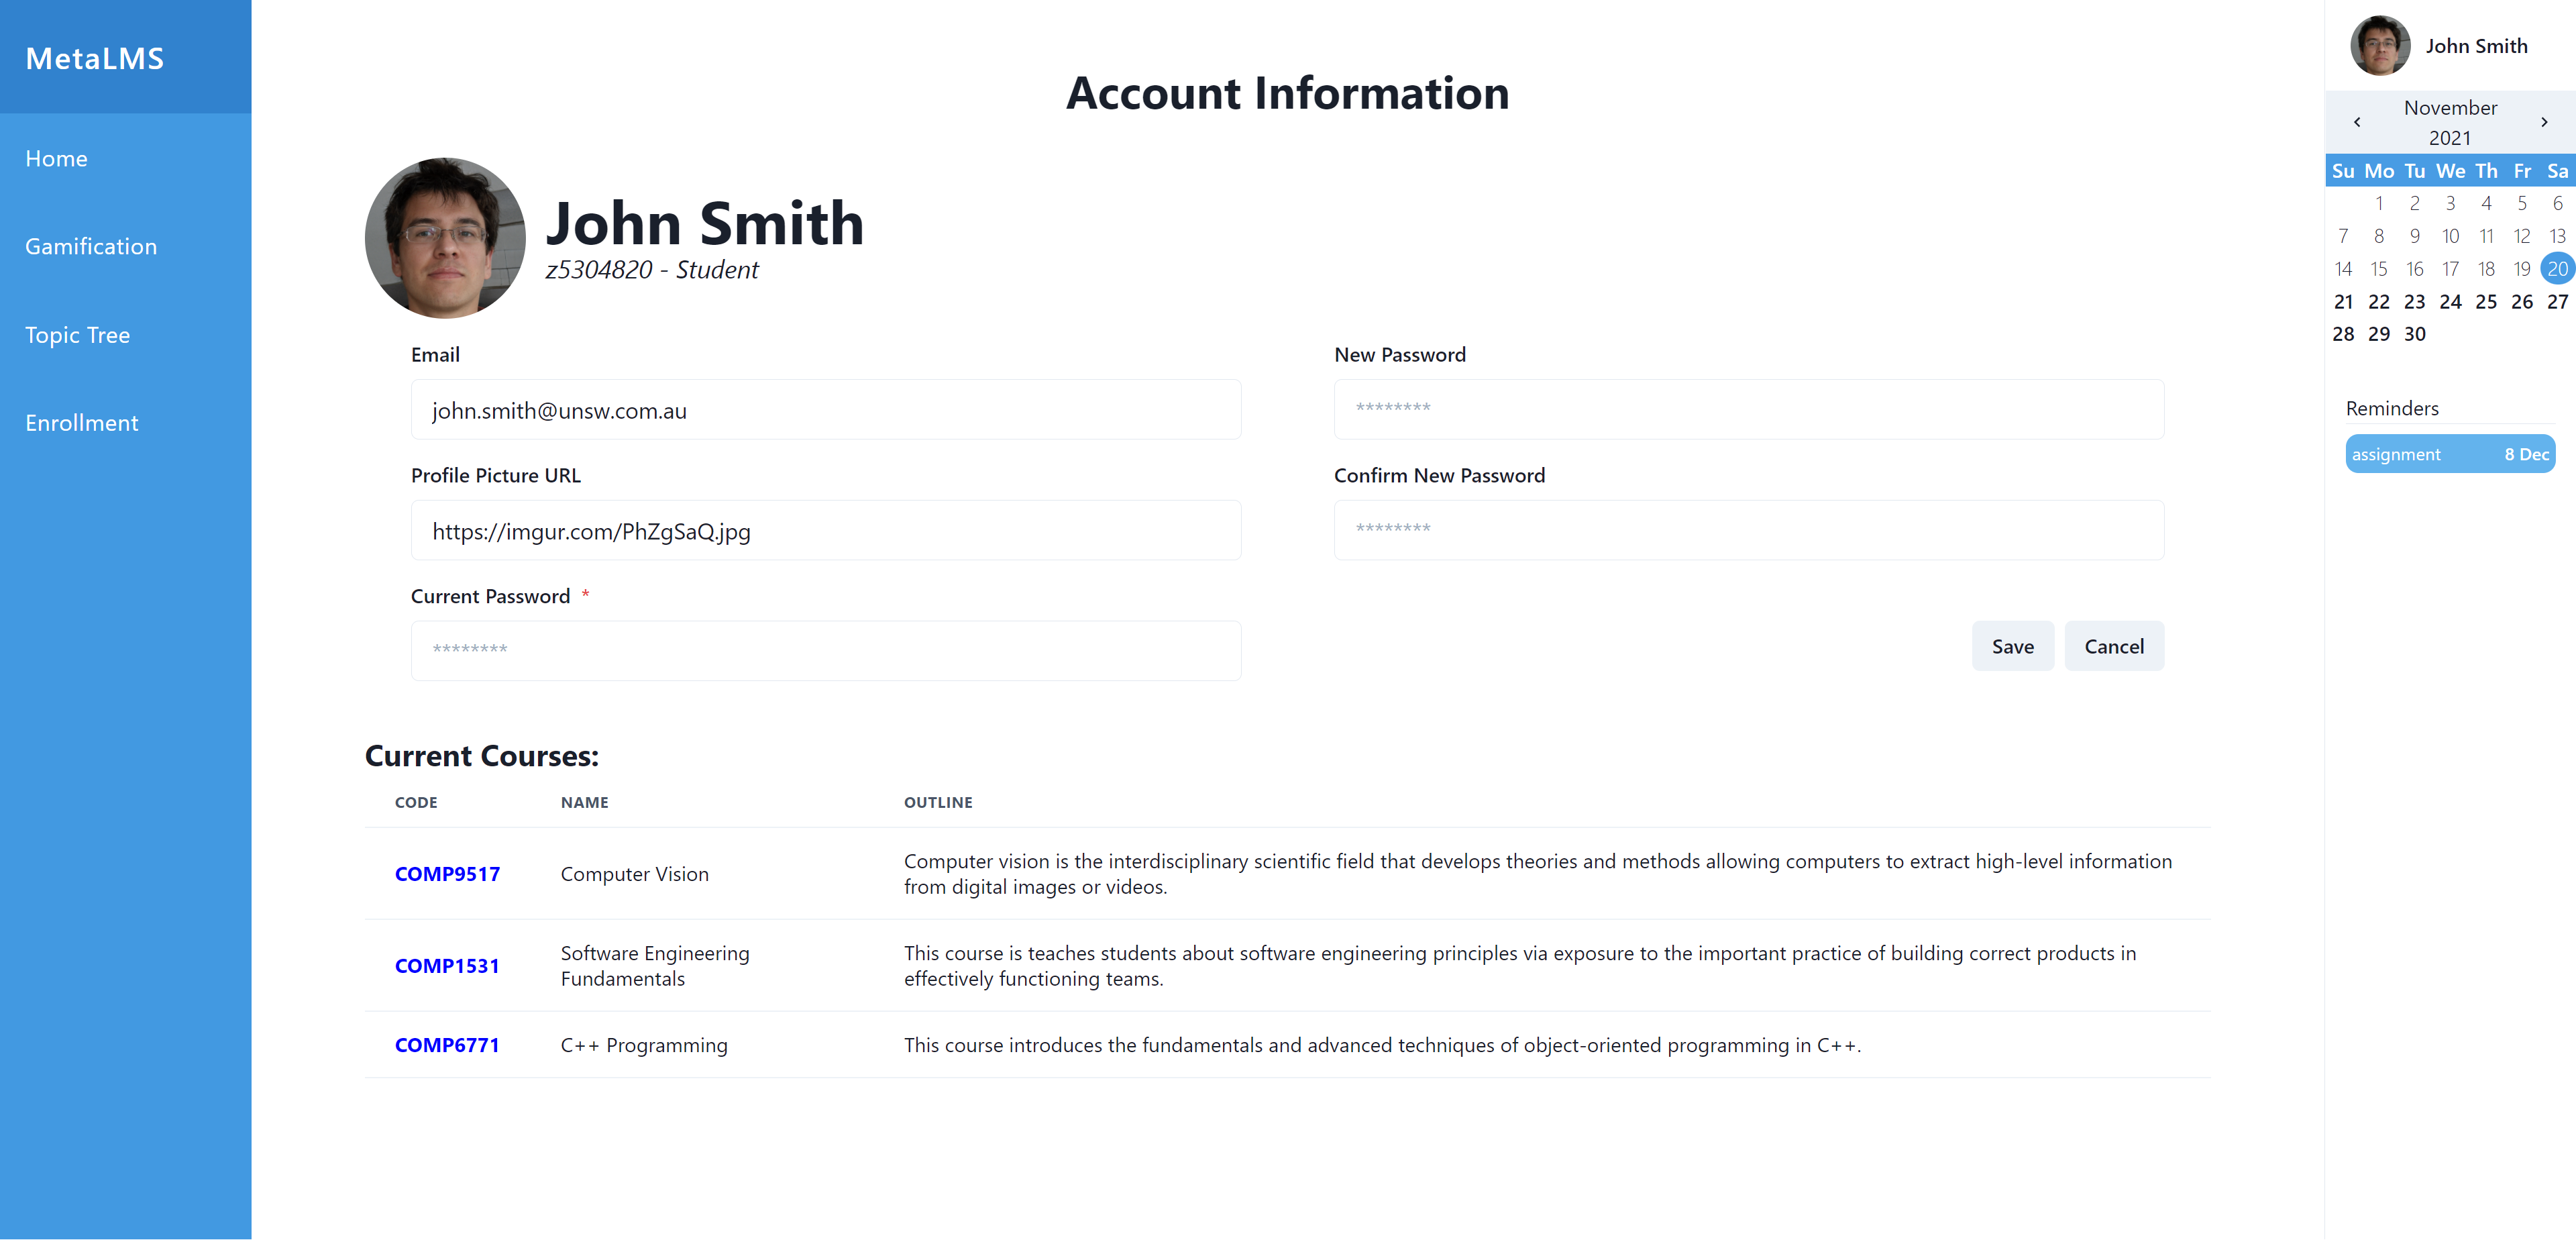
\includegraphics[scale=0.1]{images/accounts-account-management-edit.png}
    \caption{Account Editing}
\end{figure}

The current courses table allows users to at a glance view all important information regarding the courses they are currently enrolled in for student users, or managing for staff users. It shows the courses' course code, which is a hyperlink that when clicked, will take the user to that course's home page, the course's name, and the course outline, which is a brief description of what the course is about.

\textbf{How It Was Implemented}

When the page is loaded, the front-end sends a request to the back-end for all of the user's data. The back-end collects all of the personal information related to the user to send back. In the same response, it also looks at all of the courses the user is enrolled in, as the courses ID's are linked to the user's database entry. It then gathers the appropriate information for these courses and packages them into its response. This data is then reflected on the front-end.

When the user clicks the edit button, it triggers a state change on the front-end to change it to the editing state. This makes all of the text fields in the user information section editable. After the user makes their changes and clicks the save button, the front-end optimistically updates to reflect the new information while simultaneously sending a request to the backend. If the security checks pass and no other errors occur (such as the user attempting to change their email to an email in use by another user), the backend will return success. Otherwise, the backend will return an error and revert its optimistic update to the previous state and display an error toast to the user.

\textbf{Considerations}

The primary consideration for this page was security. We do not want bad actors to maliciously change a users information, so major decisions were made to prevent this. First, any changes to a users information requires the user to resubmit their current password. Failing to get this password correct will cause any changes to not be made. When updating the users password, they must not only re-enter their old password, but also confirm their new password to ensure no input errors accidentally get saved to the database.

\subsection{Enrollment Dashboard - Staff}

\textbf{Design}

For staff users, each course will have a dashboard screen that allows them to manage enrollments for that course. There are quite a few elements within the enrollment dashboard to allow staff to easily manage all enrollment features of a course from a single easy to use screen. The top portion of the page is dedicated to generating course invite codes. An invite code is a code or URL a teacher can pass onto students to allow them to enroll themselves into a course. Below that is a table that displays all currently active invite codes, how many uses they have, and how much time until they expire. It also gives action buttons that allow staff to either copy these codes to the clipboard for sharing, or to delete these codes. Beneath the table, there is a list of all currently enrolled students within the course, and all current staff of the course. There is buttons to allow staff members to manually un-enroll students. To the left of this, there is a text input form that allows staff to manually enter a students student ID and enroll them into the course. The last UI element is a toggle-able switch which sets whether a course is publicly search-able or not.

\begin{figure}[h!]
    \centering
    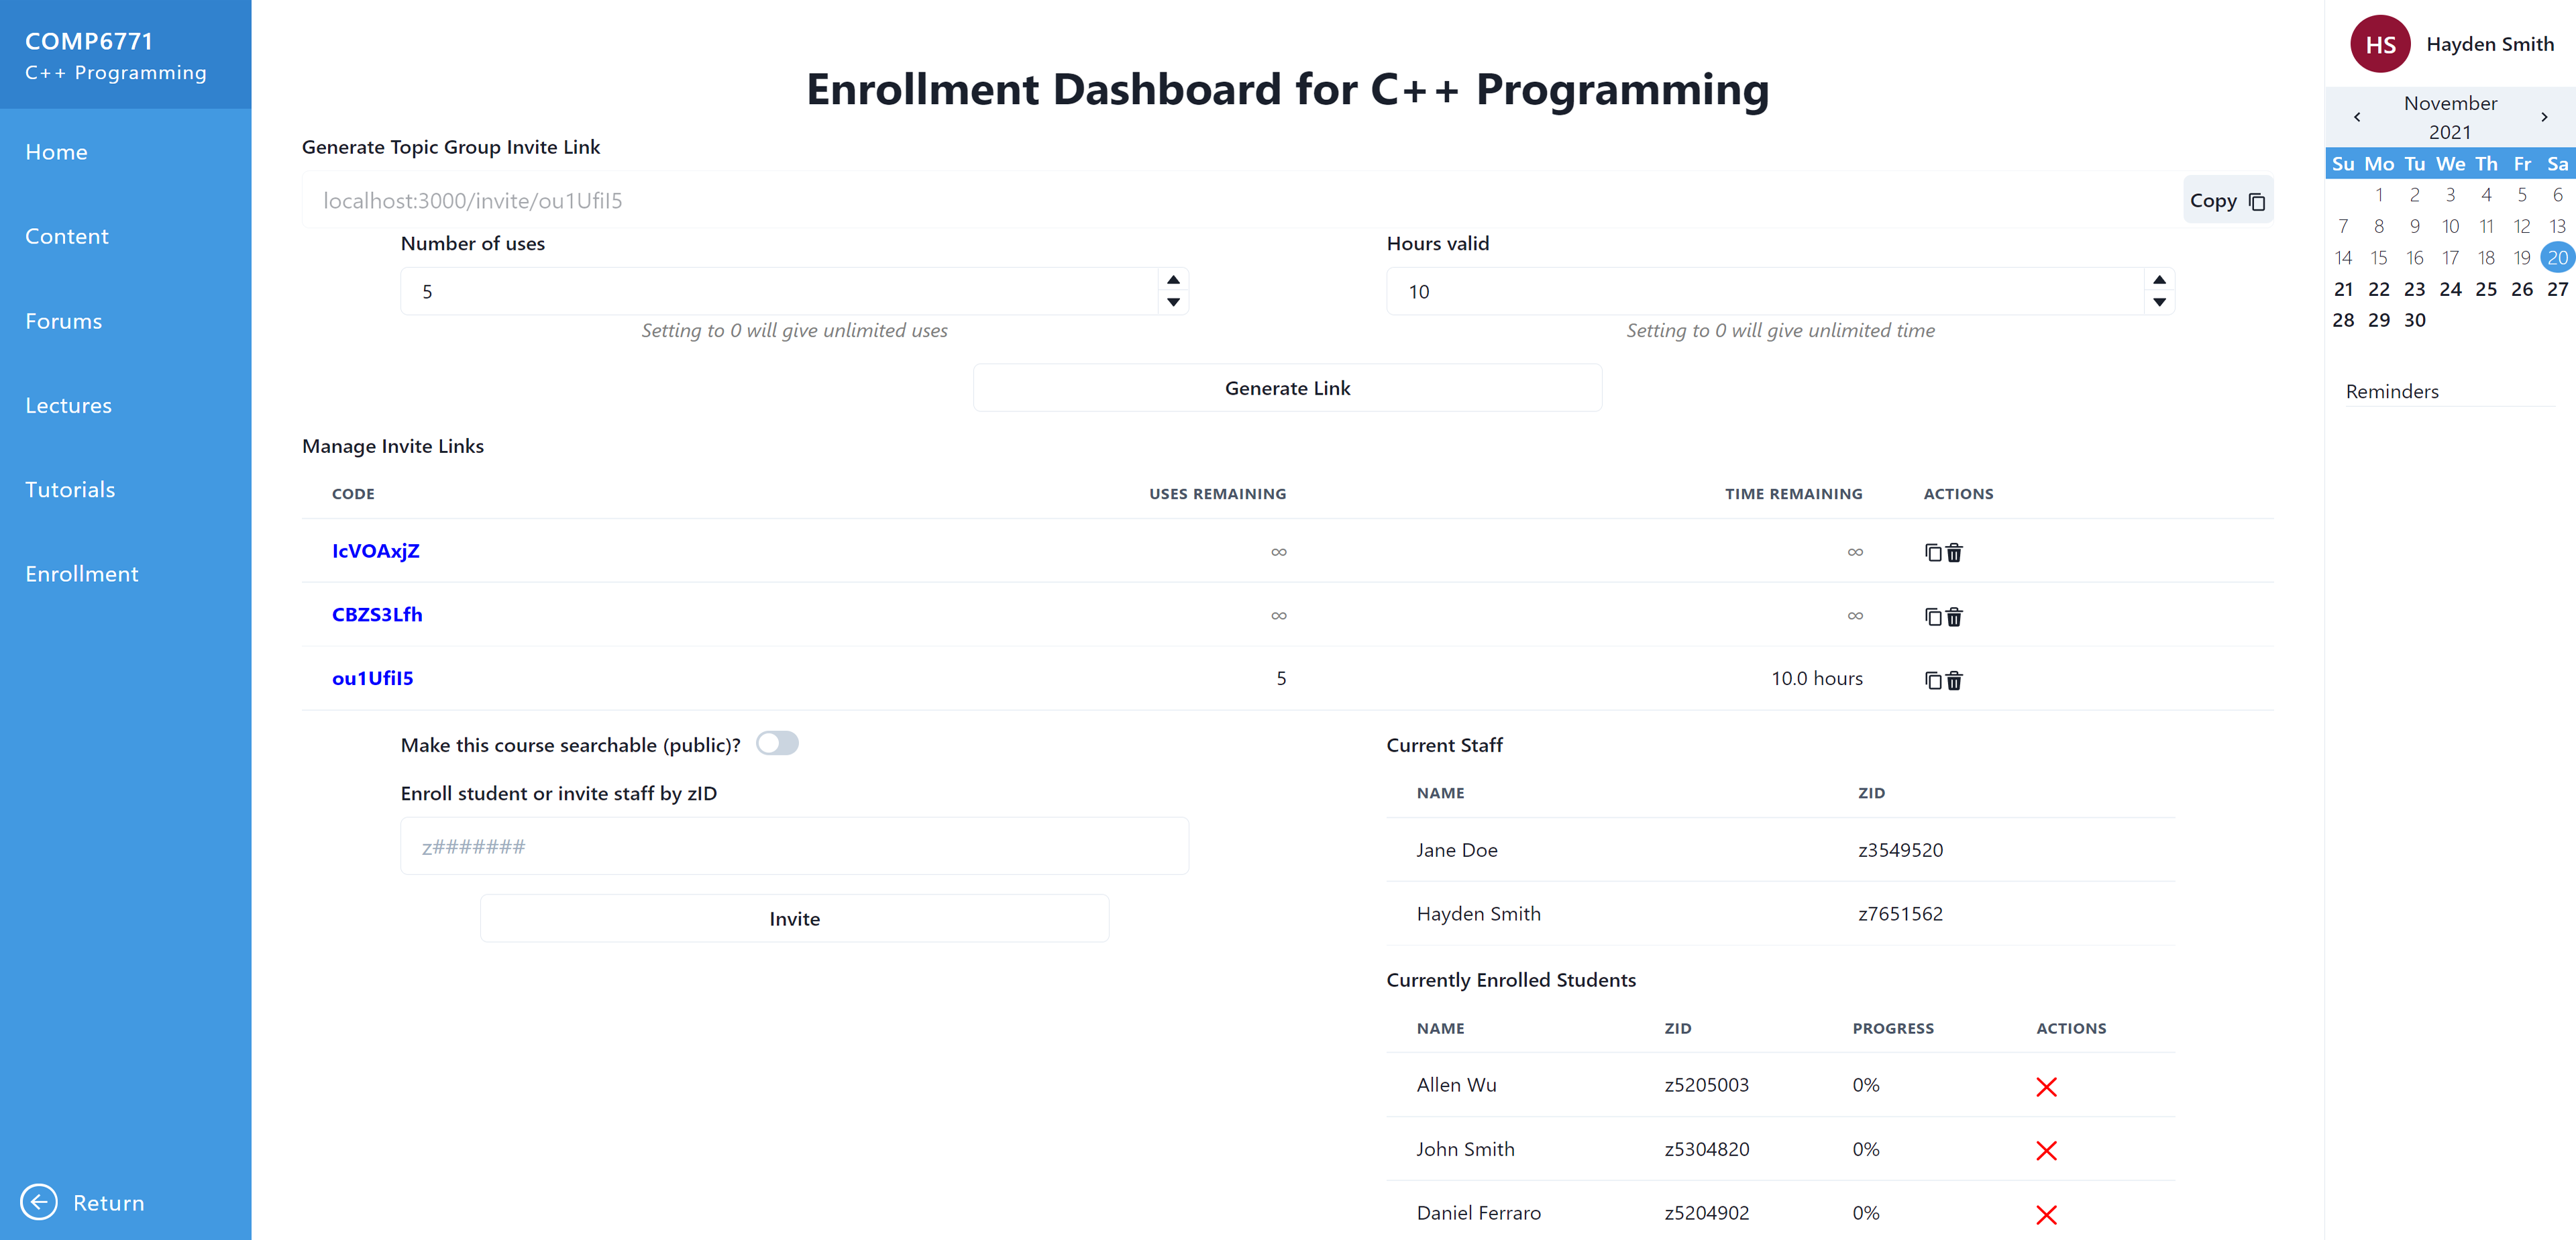
\includegraphics[scale=0.1]{images/accounts-enrollment-dashboard.png}
    \caption{Staff Enrollment Dashboard}
\end{figure}

\textbf{Purpose}

It is important to the quality of the Meta LMS that staff have a large number of tools to quickly and view and manage enrollments within a course. Due to the nature of the structure of courses as a collection of topics, and how topics are pre-requisites for other topics and as such, other topic groups, it is important for staff to be able to make changes in enrollments quickly so as to not disrupt students' learning and progress. As such, by having one central dashboard for enrollments, it gives staff a very powerful tool to quickly manage all facets of the enrollment feature, from invite codes, to manual enrollments, to search-ability.

\textbf{What Was Implemented}

This screen contains all of the important controls for managing the enrollments for a course. It required the creation of three key enrollment features, the course invite code, course search-ability, and manual enrollment by student ID. The course invite codes requires a staff member to be able to create and manage course invite codes, and manage optional parameters for these codes such as the number of uses its valid for and the time its valid for. They are also able to easily share codes with the automatic copy functionality, and delete said codes from the code management table. The search feature is very easily managed through a simple toggle switch which toggles the course between public mode, or search-able mode, and private mode, or non-search-able mode. The manual enrollment feature simply requires the staff member managing enrollments to enter the student ID of a student they wish to enroll, and submitting it. This feature also encompasses the student list, where staff can view all currently enrolled students in the course, and manually un-enroll them if they so choose.

\textbf{How It Was Implemented}

There are two options a staff member has when generating an invite code. First, they can set the number of uses a code has, with a range from zero to infinite. They can also set the time an invite code is valid for, also ranging from zero to infinite. Under the inputs for these two fields is a ``Generate Link" button which when pressed packages the values set for the optional parameters, and sends them in a request to the back-end. The back-end receives this request, and inserts a new code object into the database. If the parameter for time remaining or uses are set to 0 when sent to the back-end, the back-end does not add these parameters to the data entered into the database and thus the code has infinite uses or infinite time remaining. After entering the data for the code into the database, the backend responds to the front-end with the usable code. The front-end then automatically appends this code to the URL of the site and displays this in the text-box at the top of the screen. It also adds the code to the enrollment codes table below.

\begin{figure}[h!]
    \centering
    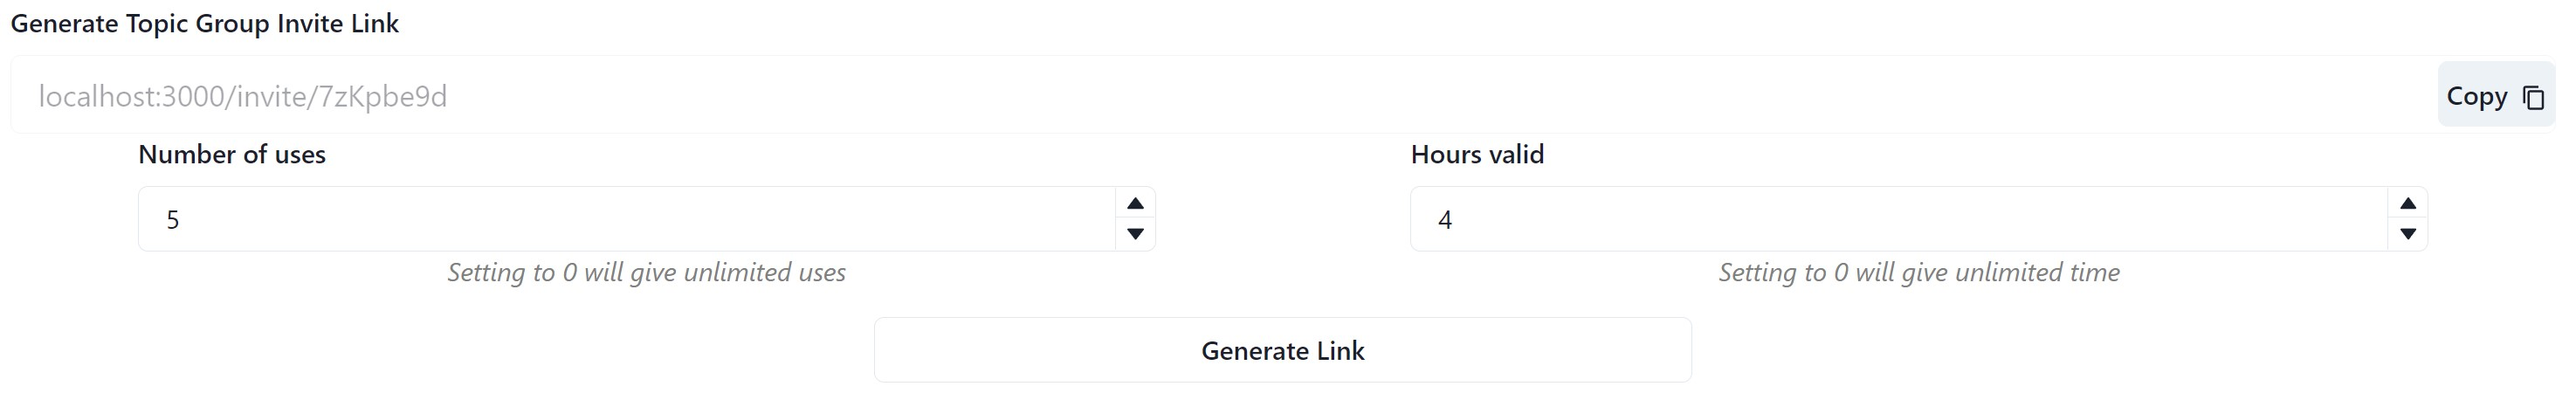
\includegraphics[scale=0.2]{images/accounts-staff-link.jpg}
    \caption{Generate Invite Link}
\end{figure}

Below the code generation area is a table where all of the currently outstanding invite links can be viewed. The data for these codes are fetched whenever the page is loaded. First, the front-end requests the list of all invite codes for the course. The back-end then gets a list of all codes for that course from the database. It then checks this list for any which have 0 uses remaining, or have 0 time remaining and deletes them from the database. It then sends this updated list to the front-end to be displayed. For these codes in the table, if the user clicks the copy button, it copies the invite link corresponding to that code directly to the clipboard. There is also a delete button, that when pressed, optimistically updates the front-end to reflect the delete, and sends a delete request to the backend, which then deletes it from the database.

\begin{figure}[h!]
    \centering
    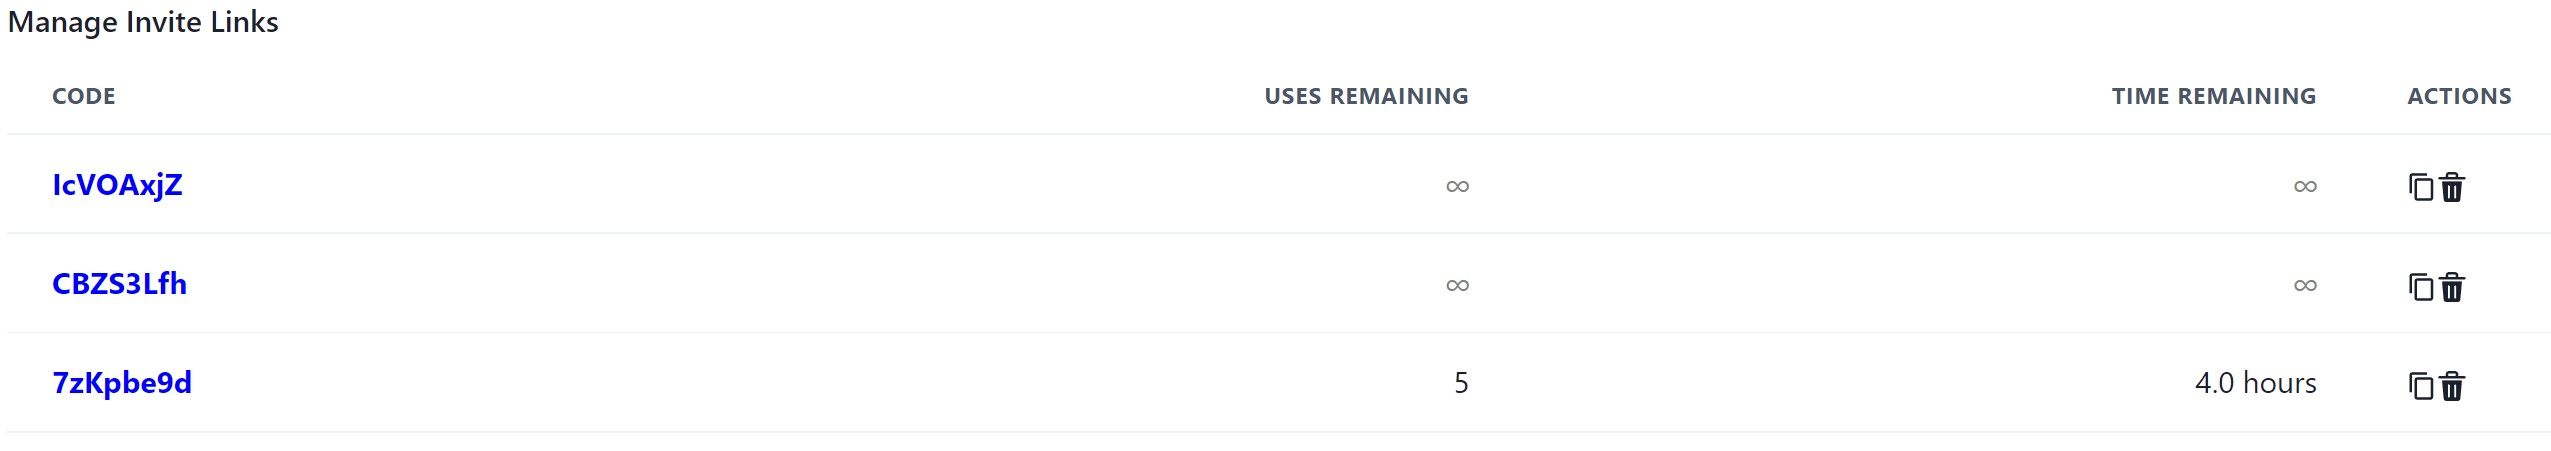
\includegraphics[scale=0.2]{images/accounts-staff-table.jpg}
    \caption{Invite Link Table}
\end{figure}

The next UI element is the search-ability toggle. On the page load, it reads the state of the search-ability of the course from the payload sent from the back-end that is requested when the page loads. It then sets the state of the search-ability toggle accordingly. When a user interacts with the toggle, the front-end optimistically updates, and sends a request to the back-end to change the state. The back-end then updates the state in the database, and sends a confirmation to the front end. 

The final component is the enroll by student ID and student list section. The enroll by student ID feature allows a staff member to enter a student's ID into the text field and submit it to be enrolled into the course. When it is submitted, the front-end checks to see if the student ID is in a valid format, and if so, sends it to the back-end to enroll the student in the course. The back-end checks to see if the student exists, then if the student is already in the course. If both of those checks pass, the back-end enters the student into the course in the database, and sends an updated enrolled student list of the course to the front-end. Unlike many other components on this page, the manual enroll is not optimistically updated on the front-end due to the higher chance of failure due to a high reliance on user input. Thus, the front-end waits to receive the updated student list from the back-end to update the student list on the front-end. The student list is simply a list of all users enrolled in the course, with students separated out from staff. A staff member will also see a red x next to all the students in the course allowing them to manually un-enroll a student. When clicked, the front-end optimistically updates the list to remove the student, then sends the delete request to the back-end, which then removes that students enrollment from the database and sends a confirmation to the front-end.

\begin{figure}[h!]
    \centering
    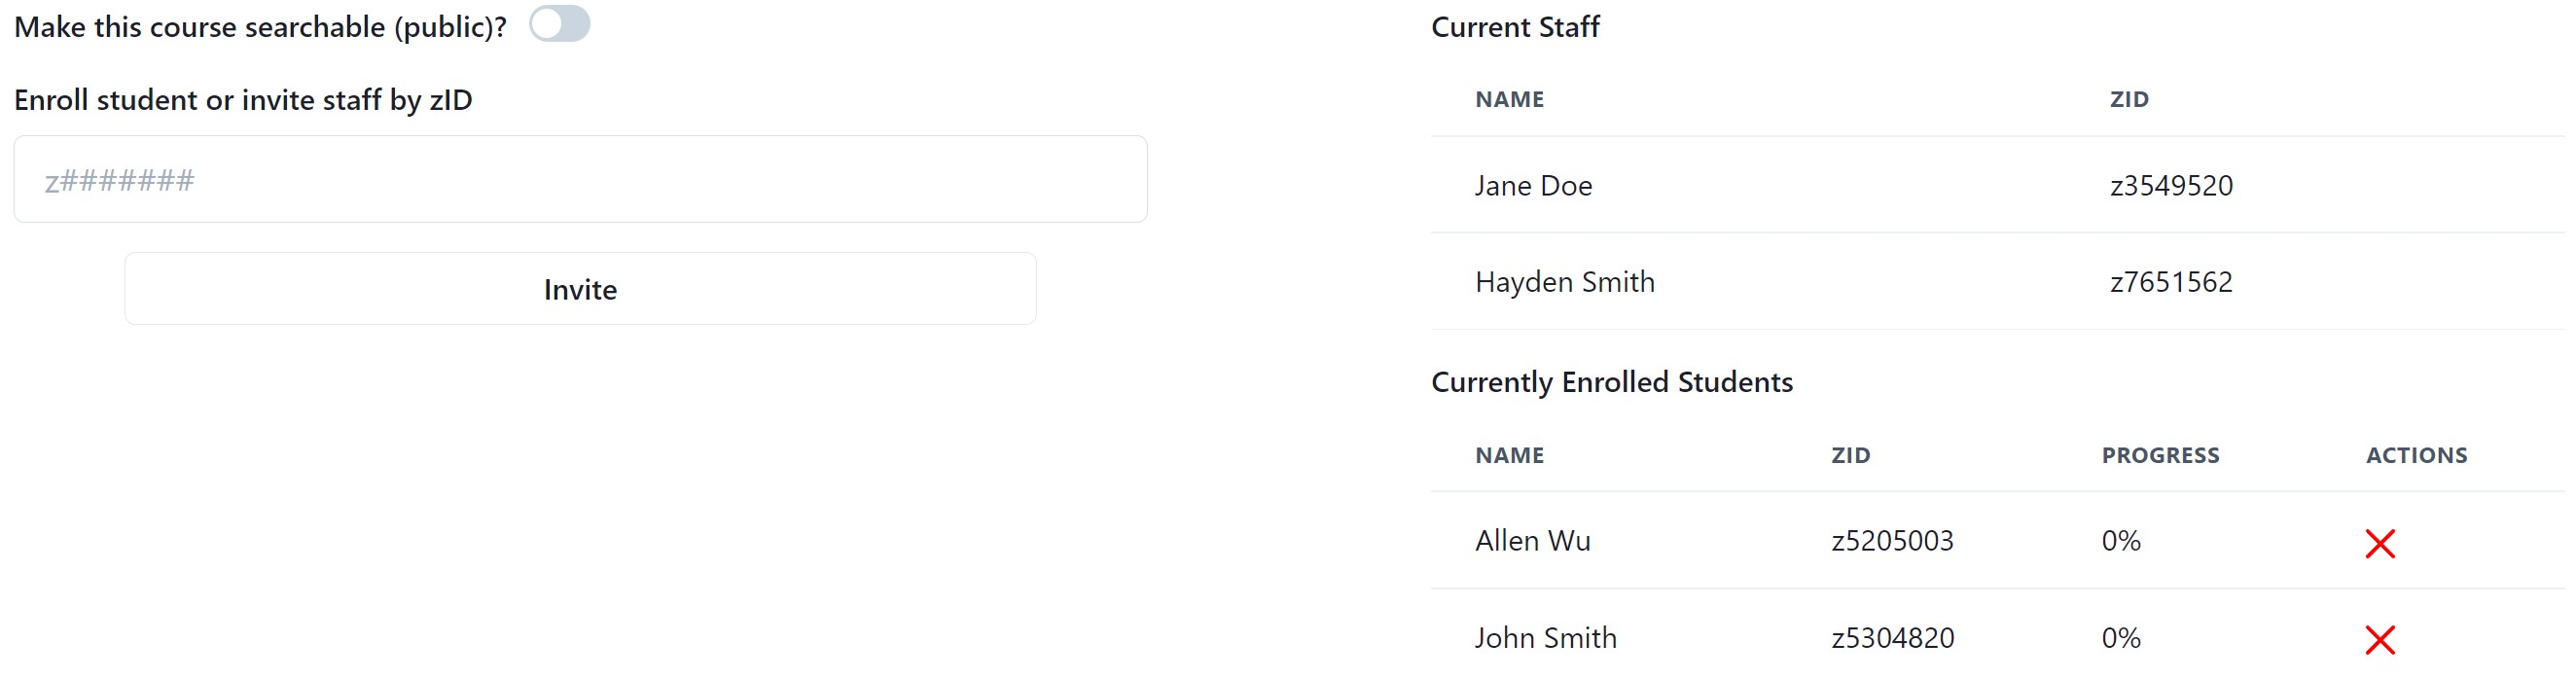
\includegraphics[scale=0.2]{images/accounts-staff-student.jpg}
    \caption{Manual Invites and Student List}
\end{figure}

For the entire page, if at any point an error occurs, any optimistic updates will be reverted, and an error toast will be displayed to the user explaining what went wrong. This is by design, so that the information on the page is always correct, and errors are in a consistent and easy to understand format.

\textbf{Considerations}

The primary consideration made when designing and developing this dashboard was ease of use. As a result, the initial plan to separate these features into multiple pages, one for invite links, one for manual invites and one for monitoring student lists and managing search-ability, was decided to not be followed in favour of the current implementation, having it all in one place. This allows users to more quickly manage enrollments, and not have to waste time switching contexts.

\subsection{Enrollment Dashboard - Student}

\textbf{Design}

The student enrollment dashboard is split into two main areas, the join with invite code area, and the search for a course area. Both sides consist of two very basic UI elements, a text input, and a submit button. For the invite code side, students input a code given to them by a teacher, and submit that to be enrolled into a course. For the search side, students can enter either the course code, course name, or key words related to something they wish to learn about and submit it. This will then return matching courses in the form of cards, which say the courses name, code and course outline, and has a button they can press to enroll.

\begin{figure}[h!]
    \centering
    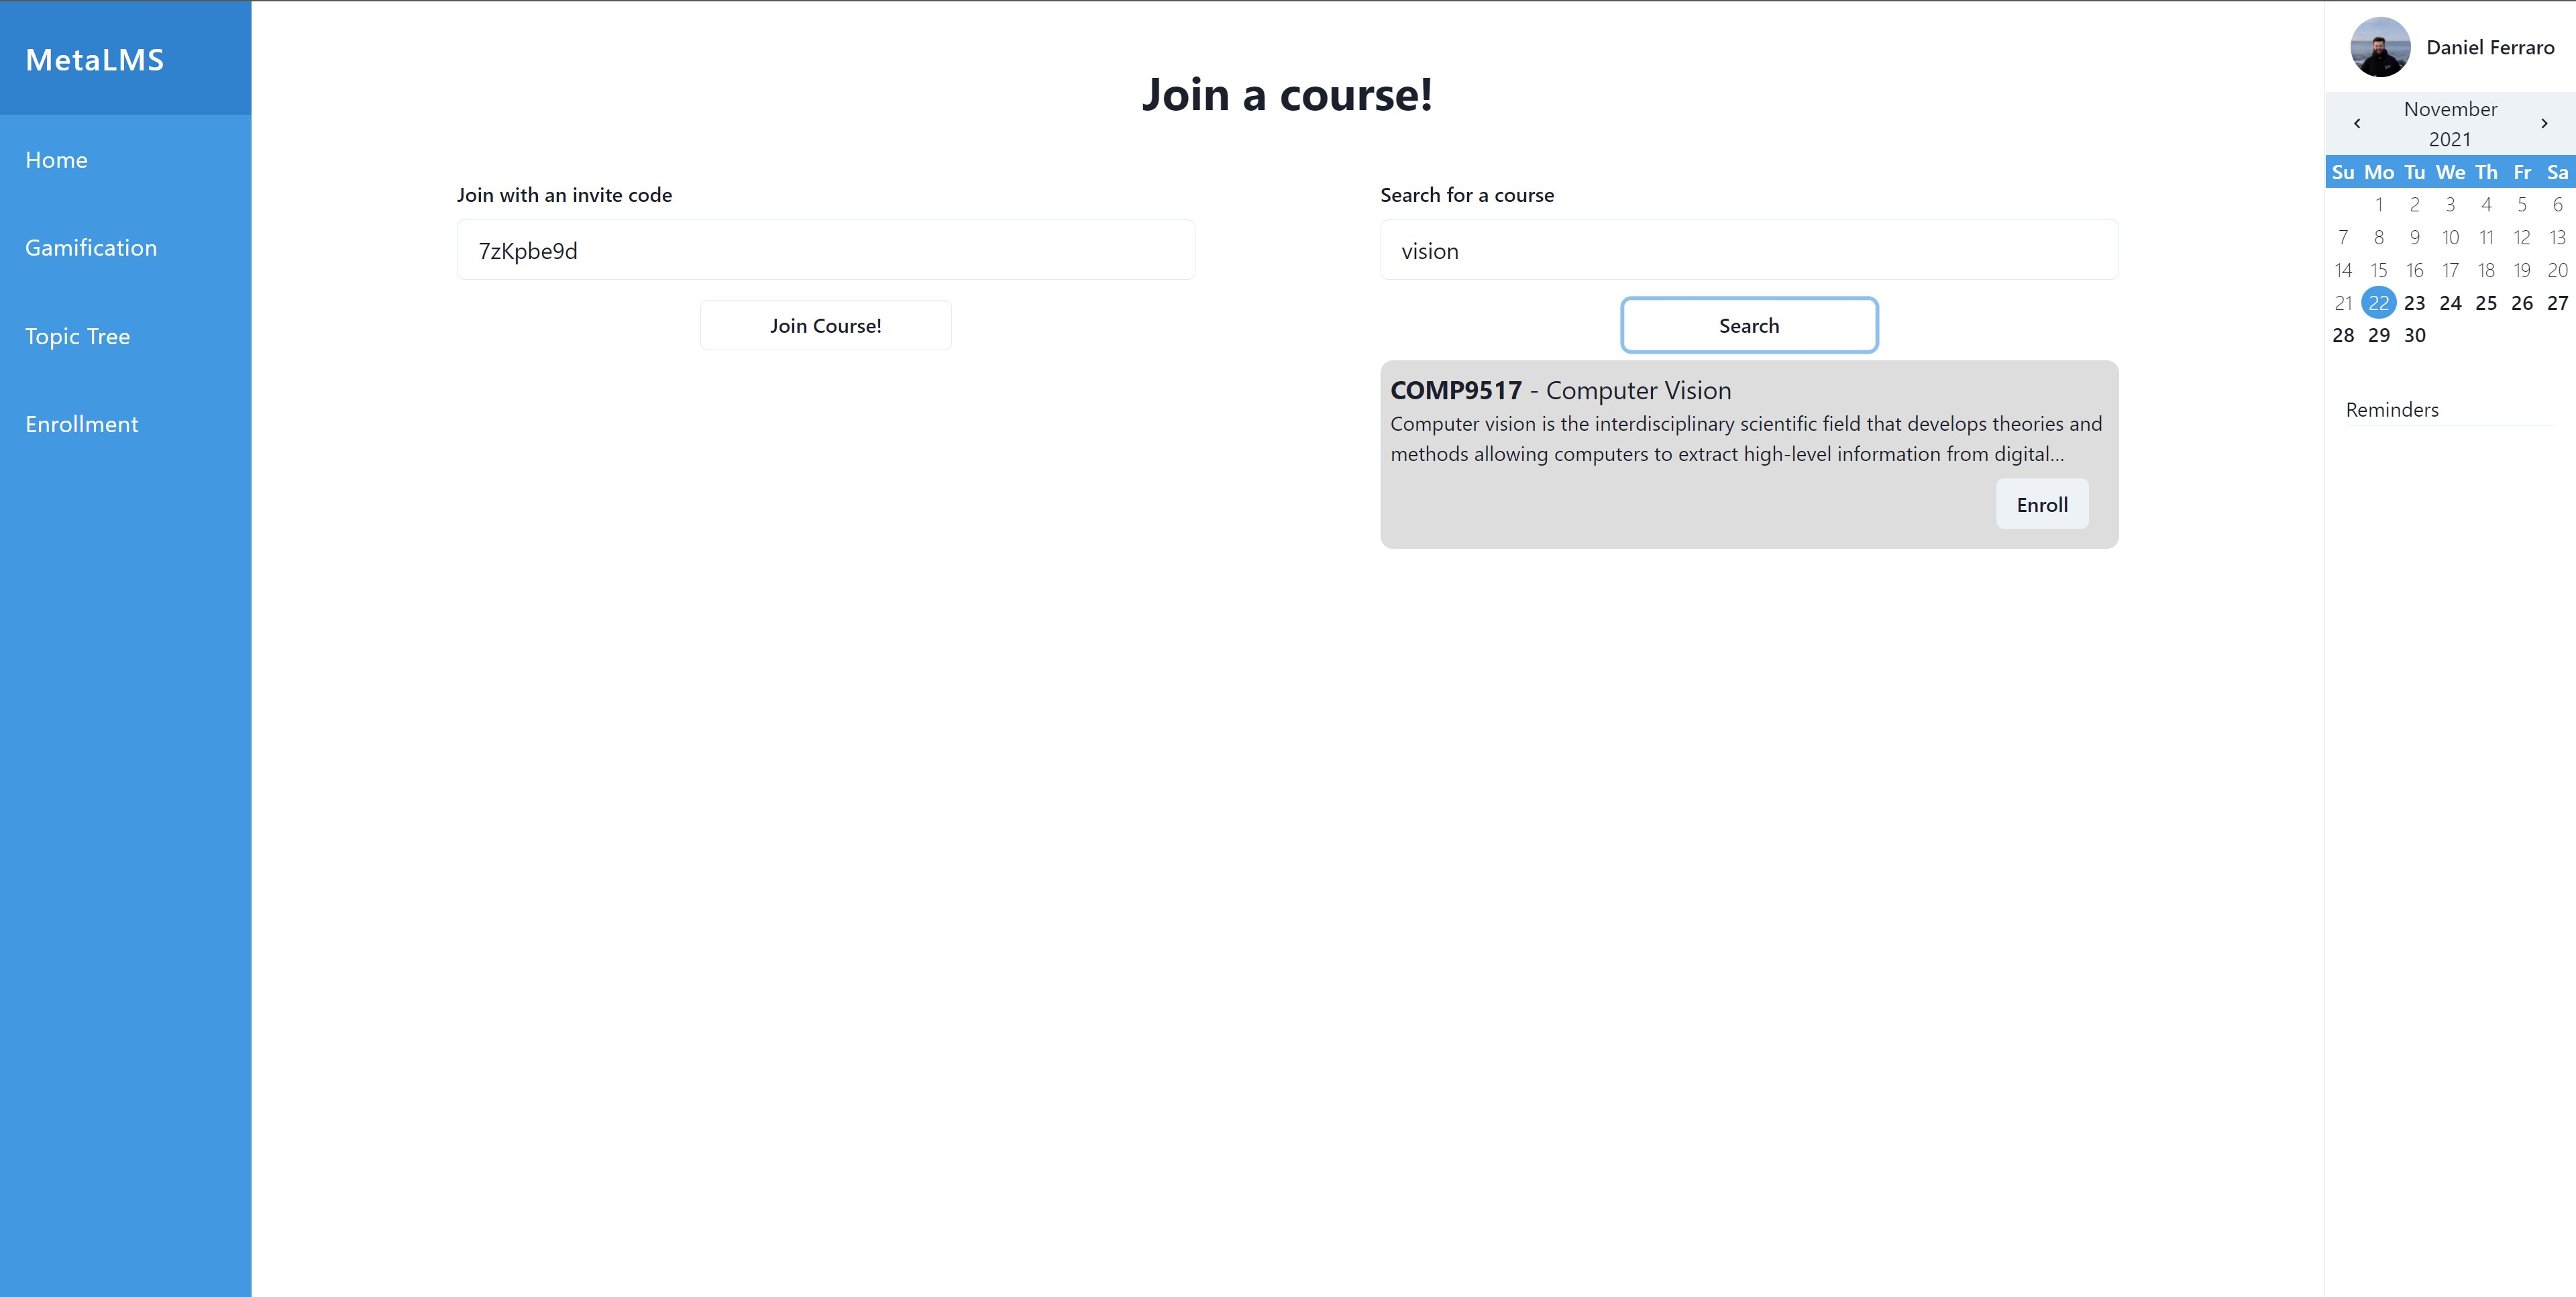
\includegraphics[scale=0.1]{images/accounts-student-dash.jpg}
    \caption{Student Enrollment Dashboard}
\end{figure}

\textbf{Purpose}

Due to the fast-paced nature of learning that comes from using the topic group approach, it is important that students have a high level of agency over their learning. As such, it is essential the tools students have access to that allow them to manage their enrollments are powerful enough to afford them this agency. This adds a tremendous amount of value to the Meta LMS as it gives students access to the full benefits of the topic group system.

\textbf{What Was Implemented}

The two systems implemented are the student face of the invite code system, and the course searching system. The course invite system also encapsulates the login redirect feature, that allows students who are not currently logged in to the LMS to simply click an invite link, login or sign up, and then automatically be redirected to the student enrollment dashboard with the invite code pre-filled to quickly and easily begin using the LMS to learn.

\textbf{How It Was Implemented}

The course invite system works by allowing a user to input a course invite code, and submit it to enroll themselves into a course. This field will be blank on the page load if the user has navigated to the enrollment page manually, but will be pre-filled if the user has arrived to the page by using an invite link. This is done by reading the ID URL parameter of the invite link, and setting that as the default value of that text field. When the user submits an invite code, the front-end sends that code in a request to the back-end. The back-end first checks to see if the code exists in the database, then checks if the code is valid, that is, if it has time remaining, or uses remaining. If the code has become invalid, it deletes it from the database and sends an error to the front-end. If the code is valid, it then checks if the student is already enrolled in the course, and if they aren't, it enrolls them, and updates the remaining uses for that invite. If the student's enrollment causes this code to become invalid, it is then removes that code from the database. Once the enrollment is successful, its sends the confirmation payload to the front-end. This payload contains the information of the course the student was enrolled in, as well as the confirmation status. This information is then displayed to the user on the front-end in the form of a toast that confirms the enrollment was successful and the course they were enrolled in.

The search for a course feature is much the same, the user inputs a string and sends it to the back-end. However, the string entered will correspond to either a course's code, a course title or details about a course. When the user submits this, the front-end sends a request to the back-end for results related to the user's query. The back-end then compares the query to the course codes, names and course outlines stored in the back-end, but only of courses that have been marked as search-able. It then assembles a list of results and sends that response back to the front-end. The front-end then displays this list to the user in the form of cards. These cards contain all the basic information about the course, and also have an enroll button. When the user clicks the enroll button, the front-end sends the enroll request to the back-end. The back-end then does checks to see if the user is already in the course, and if not, enrolls them in the course and sends confirmation back to the front-end. This successful enrollment is then displayed in the form of a toast.

\begin{figure}[h!]
    \centering
    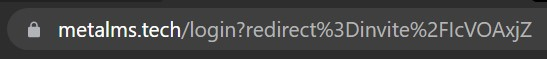
\includegraphics[scale=0.6]{images/accounts-login-redirect.jpg}
    \caption{Invite Code Login Redirect}
\end{figure}

The feature that handles the redirect to the invite screen from the login page does so by storing the invite code from an invite link in the redirect URL parameter of the invite page. If this parameter is present, once a user has successfully logged in, it will redirect them to the invite page and pre-fill the code.

\textbf{Considerations}

The primary consideration for this feature was the redirect from the login screen, particularly for new users. To create as positive a user experience as possible, the sign up to enrollment process needs to be as seamless and friction-less as possible. Allowing users to simply input an invite code, create an account then automatically be redirected to the enrollment page with the code pre-filled makes this enrollment process as easy as possible for the user, allowing them to begin using the LMS to learn very quickly.